\section{Sơ đồ thực thể -- mối kết hợp (ERD)}

Mô hình quan niệm được biểu diễn bằng sơ đồ thực thể -- mối kết hợp theo ký pháp Chen (Hình~\ref{fig:erd}). Sơ đồ gồm 11 thực thể và 16 mối kết hợp, ứng với các mối quan hệ đã phân tích ở mục 2.2. Để sơ đồ dễ đọc, mỗi thực thể chỉ thể hiện thuộc tính khóa và hai thuộc tính tiêu biểu; danh sách thuộc tính đầy đủ nằm ở mục 2.1.

\begin{figure}[!htb]
    \centering
    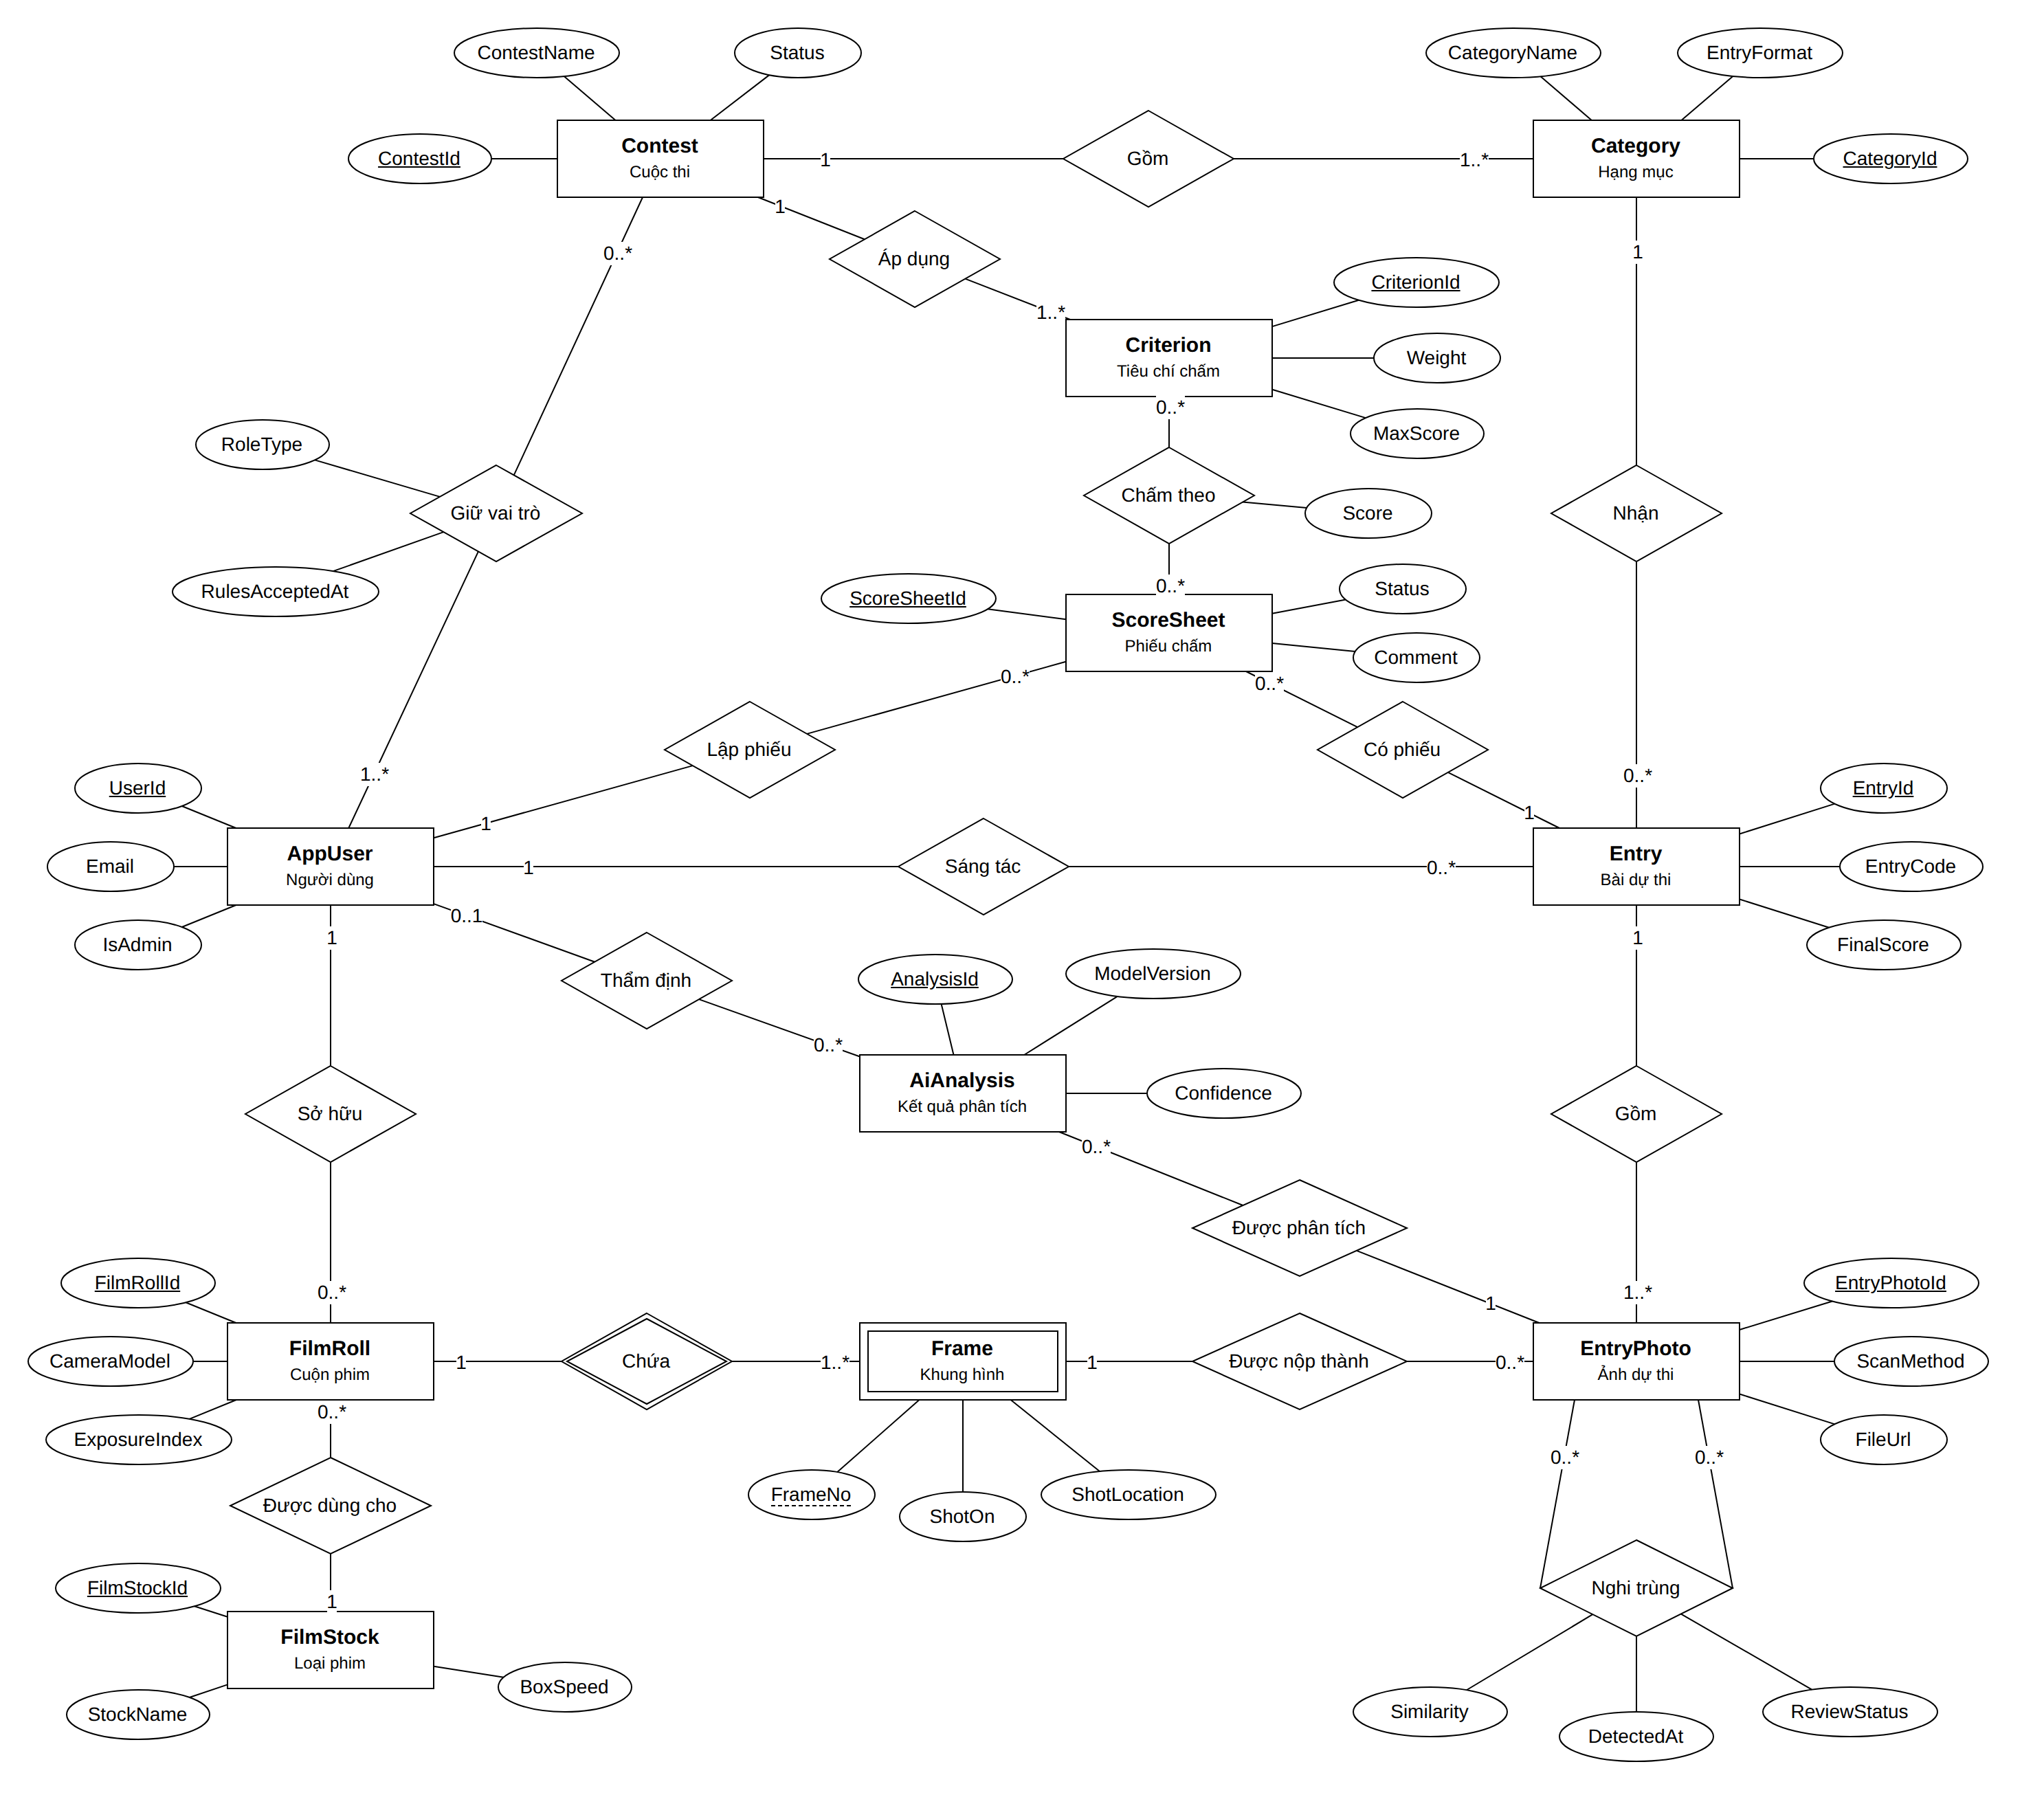
\includegraphics[width=\textwidth]{images/So_do_khai_niem.png}
    \caption{Sơ đồ thực thể -- mối kết hợp mức quan niệm (Conceptual ERD)}
    \label{fig:erd}
\end{figure}

\subsection{Quy ước ký hiệu}

\begin{itemize}
    \item Hình chữ nhật là thực thể; hình chữ nhật đôi là thực thể yếu (\texttt{Frame}).
    \item Hình thoi là mối kết hợp; hình thoi đôi là mối kết hợp định danh (Chứa), nối thực thể yếu với thực thể chủ của nó.
    \item Hình elip là thuộc tính. Thuộc tính gạch dưới là khóa; thuộc tính gạch dưới nét đứt là khóa cục bộ của thực thể yếu (\texttt{FrameNo}).
    \item Bản số ghi ở đầu đường nối, cạnh thực thể, theo dạng tối thiểu..tối đa: 1 là đúng một, 0..1 là không hoặc một, 0..* là không hoặc nhiều, 1..* là ít nhất một. Con số đặt cạnh thực thể nào cho biết số thể hiện của thực thể đó ứng với một thể hiện ở phía bên kia. Ví dụ, 1..* đặt cạnh \texttt{Category} trên mối kết hợp Gồm nghĩa là mỗi cuộc thi có ít nhất một hạng mục.
\end{itemize}

\subsection{Các lựa chọn mô hình hóa}

\begin{itemize}
    \item Ba mối kết hợp nhiều--nhiều Giữ vai trò, Chấm theo và Nghi trùng mang thuộc tính riêng, nên được vẽ thành hình thoi kèm elip. Ở mục 2.1 chúng được liệt kê cùng các thực thể để thấy đủ thuộc tính; khi chuyển sang lược đồ logic ở Chương 3, mỗi mối kết hợp này trở thành một bảng: \texttt{ContestRole}, \texttt{ScoreDetail} và \texttt{DuplicateMatch}.
    \item Phiếu chấm có vòng đời riêng, từ nháp đến chốt, và còn tham gia mối kết hợp Chấm theo với tiêu chí. Vì vậy phiếu chấm được mô hình hóa thành thực thể \texttt{ScoreSheet}, nối với bài dự thi qua mối kết hợp Có phiếu và với giám khảo qua mối kết hợp Lập phiếu, thay vì chỉ là một mối kết hợp giữa bài dự thi và giám khảo.
    \item \texttt{Frame} là thực thể yếu: số khung chỉ có nghĩa trong phạm vi một cuộn, nên khung được định danh bằng khóa của \texttt{FilmRoll} cộng với khóa cục bộ \texttt{FrameNo}.
    \item Nghi trùng là mối kết hợp đệ quy: hai đường nối cùng xuất phát từ \texttt{EntryPhoto}, ứng với ảnh thứ nhất và ảnh thứ hai của một cặp.
    \item \texttt{AppUser} tham gia năm mối kết hợp ứng với năm vai trò: giữ vai trò trong cuộc thi, sở hữu cuộn phim, sáng tác bài dự thi, lập phiếu chấm và thẩm định kết quả phân tích.
\end{itemize}

\subsection{Bản số và mức tham gia}

Bảng dưới đây ghi bản số của từng mối kết hợp theo thứ tự hai thực thể ở cột thứ hai.

\begin{longtable}{|L{2.5cm}|L{3.5cm}|L{1.9cm}|L{6.1cm}|}
\caption{Bản số và mức tham gia của các mối kết hợp} \label{tab:ban-so} \\
\hline
\textbf{Mối kết hợp} & \textbf{Thực thể} & \textbf{Bản số} & \textbf{Diễn giải} \\ \hline
\endfirsthead
\hline
\textbf{Mối kết hợp} & \textbf{Thực thể} & \textbf{Bản số} & \textbf{Diễn giải} \\ \hline
\endhead
Gồm & \texttt{Contest} -- \texttt{Category} & 1 -- 1..* & Mỗi cuộc thi có ít nhất một hạng mục; mỗi hạng mục thuộc đúng một cuộc thi. \\ \hline
Áp dụng & \texttt{Contest} -- \texttt{Criterion} & 1 -- 1..* & Mỗi cuộc thi có ít nhất một tiêu chí chấm; mỗi tiêu chí thuộc đúng một cuộc thi. \\ \hline
Giữ vai trò & \texttt{AppUser} -- \texttt{Contest} & 1..* -- 0..* & Mỗi cuộc thi có ít nhất một người giữ vai trò (ban tổ chức); một người có thể giữ vai trò ở nhiều cuộc thi hoặc chưa ở cuộc thi nào. Thuộc tính: RoleType, RulesAcceptedAt. \\ \hline
Sở hữu & \texttt{AppUser} -- \texttt{FilmRoll} & 1 -- 0..* & Mỗi cuộn phim có đúng một chủ; một thí sinh có thể có nhiều cuộn. \\ \hline
Được dùng cho & \texttt{FilmStock} -- \texttt{FilmRoll} & 1 -- 0..* & Mỗi cuộn dùng đúng một loại phim; một loại phim có thể chưa được cuộn nào dùng. \\ \hline
Chứa (định danh) & \texttt{FilmRoll} -- \texttt{Frame} & 1 -- 1..* & Mỗi khung thuộc đúng một cuộn; một cuộn được khai báo khi có ít nhất một khung. \\ \hline
Được nộp thành & \texttt{Frame} -- \texttt{EntryPhoto} & 1 -- 0..* & Mỗi ảnh dự thi là đúng một khung; một khung có thể được nộp nhiều lần hoặc chưa được nộp. \\ \hline
Nhận & \texttt{Category} -- \texttt{Entry} & 1 -- 0..* & Mỗi bài dự thi thuộc đúng một hạng mục. \\ \hline
Sáng tác & \texttt{AppUser} -- \texttt{Entry} & 1 -- 0..* & Mỗi bài dự thi có đúng một tác giả. \\ \hline
Gồm & \texttt{Entry} -- \texttt{EntryPhoto} & 1 -- 1..* & Mỗi bài có ít nhất một ảnh; mỗi ảnh dự thi thuộc đúng một bài. \\ \hline
Có phiếu & \texttt{Entry} -- \texttt{ScoreSheet} & 1 -- 0..* & Mỗi phiếu chấm đúng một bài; một bài có thể có phiếu của nhiều giám khảo. \\ \hline
Lập phiếu & \texttt{AppUser} -- \texttt{ScoreSheet} & 1 -- 0..* & Mỗi phiếu chấm thuộc đúng một giám khảo. \\ \hline
Chấm theo & \texttt{ScoreSheet} -- \texttt{Criterion} & 0..* -- 0..* & Một phiếu chấm theo nhiều tiêu chí; phiếu nháp có thể chưa có điểm. Thuộc tính: Score. \\ \hline
Được phân tích & \texttt{EntryPhoto} -- \texttt{AiAnalysis} & 1 -- 0..* & Mỗi kết quả phân tích thuộc đúng một ảnh; một ảnh có thể được phân tích nhiều lần. \\ \hline
Thẩm định & \texttt{AppUser} -- \texttt{AiAnalysis} & 0..1 -- 0..* & Mỗi kết quả có tối đa một người thẩm định; kết quả chưa thẩm định thì chưa có người thẩm định. \\ \hline
Nghi trùng (đệ quy) & \texttt{EntryPhoto} -- \texttt{EntryPhoto} & 0..* -- 0..* & Một ảnh có thể nghi trùng với nhiều ảnh khác; mỗi cặp chỉ ghi một lần. Thuộc tính: Similarity, DetectedAt, ReviewStatus. \\ \hline
\end{longtable}

Các giá trị tối thiểu bằng 1 ở phía \textquotedblleft nhiều\textquotedblright{}, như mỗi cuộc thi có ít nhất một hạng mục hay mỗi bài có ít nhất một ảnh, là quy tắc nghiệp vụ. Khóa ngoại chỉ bảo đảm được phía \textquotedblleft một\textquotedblright{}, nên các ràng buộc tối thiểu này được kiểm tra ở tầng dịch vụ khi cuộc thi mở hoặc khi bài dự thi được nộp.
